\documentclass[convert={density=300,outext=.png}]{standalone}
\usepackage{tikz}
\usetikzlibrary{shapes,arrows,decorations,decorations.pathmorphing,arrows.meta,patterns,decorations.markings}

\begin{document}
%% Use \usepackage{tikz}
%% Use \usetikzlibrary{shapes,arrows,decorations, decorations.pathmorphing,arrows.meta,patterns}
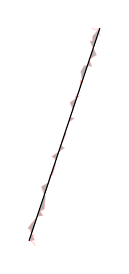
\begin{tikzpicture}[scale=0.9000]
	\tikzstyle{every node}=[scale=1.0000]
	
	%%Created with tikzpy
	
	\draw [<-> ,line width = 0.2000 ,decorate, decoration={random steps, segment length=2, amplitude=2} ,red!30 , fill= black!30 ,]  (1.0000,2.0000,0.0000) -- (2.0000,5.0000,0.0000);
	\draw  (1.0000,2.0000,0.0000) -- (2.0000,5.0000,0.0000);

\end{tikzpicture}
\end{document}
